\documentclass[10pt,xcolor=pdflatex]{beamer}
\usepackage{newcent}
\usepackage[utf8]{inputenc}
%\usepackage[czech]{babel}
\usepackage{hyperref}
\usepackage{fancyvrb}
\usepackage{multicol}

\usetheme{FIT}

%%%%%%%%%%%%%%%%%%%%%%%%%%%%%%%%%%%%%%%%%%%%%%%%%%%%%%%%%%%%%%%%%%
\title{Continuous Integration and Automated Code Review in Open Source Projects}

\author[]{Adrián Tóth}

\institute[]{
	Brno University of Technology, Faculty of Information Technology\\
	Bo\v{z}et\v{e}chova 1/2. 612 66 Brno - Kr\'alovo Pole\\
	xtotha01@fit.vutbr.cz
	}

%\date{January 1, 2016}
%\date{\today}
\date{} % bez data

%%%%%%%%%%%%%%%%%%%%%%%%%%%%%%%%%%%%%%%%%%%%%%%%%%%%%%%%%%%%%%%%%%

\begin{document}

\frame[plain]{\titlepage}

\begin{frame}\frametitle{Introduction}
    What is \textit{Continuous Integration}?\\[1em]
    What is \textit{Automated Code Review}?\\[1em]
    Where is it used and why?\\[1em]
    How it works?
\end{frame}

\begin{frame}\frametitle{Continuous Integration}
	\begin{itemize}
		\item common part of fast software development\\[1em]
		\item adaptive development technique\\[1em]
		\item reduce integration problems\\[1em]
		\item integrations are verified via automated tests and builds\\[1em]
		\item popular in open source projects which are frequently developed by a group of people\\[1em]
		\item available CI services: \textit{Travis CI}, \textit{Jenkins}, \textit{TeamCity}, ...
	\end{itemize}
\end{frame}

\begin{frame}\frametitle{Continuous Integration}
	\begin{centering}
		\large{Components of continuous integration system}\\
	\end{centering}
	\begin{figure}[H]
		\centering
		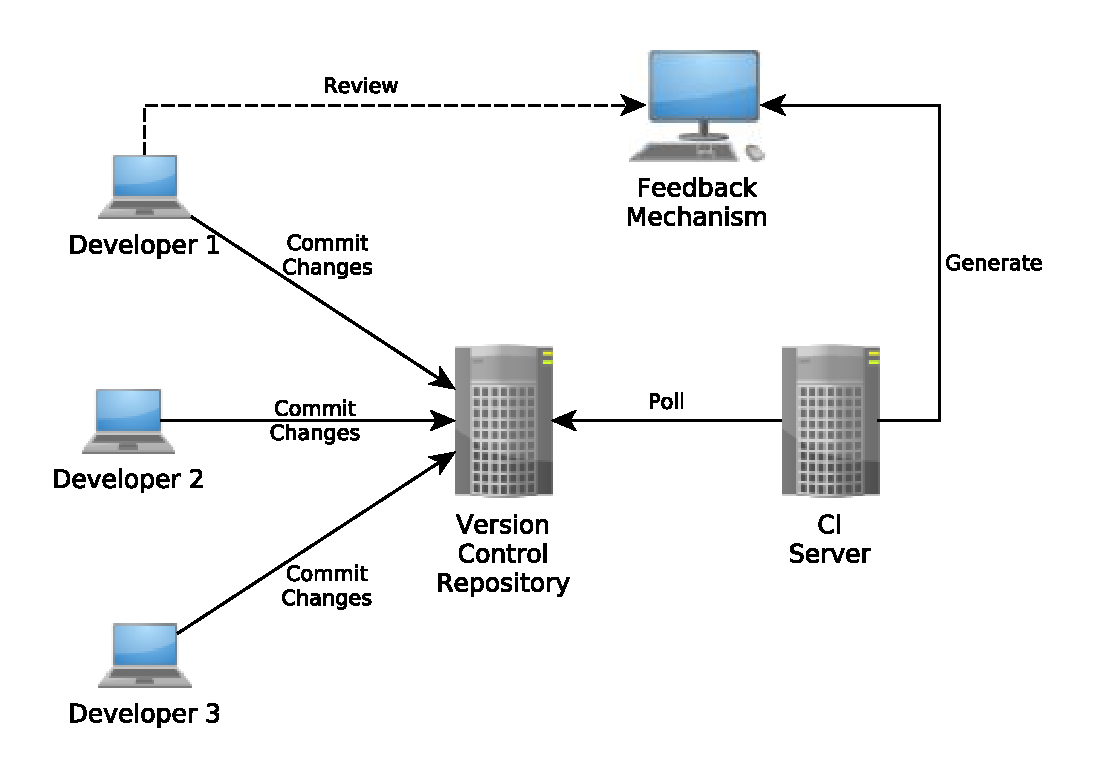
\includegraphics[scale=0.5]{eps/components_of_CI_system.eps}
	\end{figure}
\end{frame}

\begin{frame}\frametitle{Continuous Integration}
	\begin{centering}
		\large{The basics of CI}\\[1em]
	\end{centering}
	\begin{multicols}{2}
		Stages of CI:
		\begin{enumerate}
			\item The change
			\item The reaction
			\item The feedback
			\item The waiting 
		\end{enumerate}
		\begin{figure}[H]
			\centering
			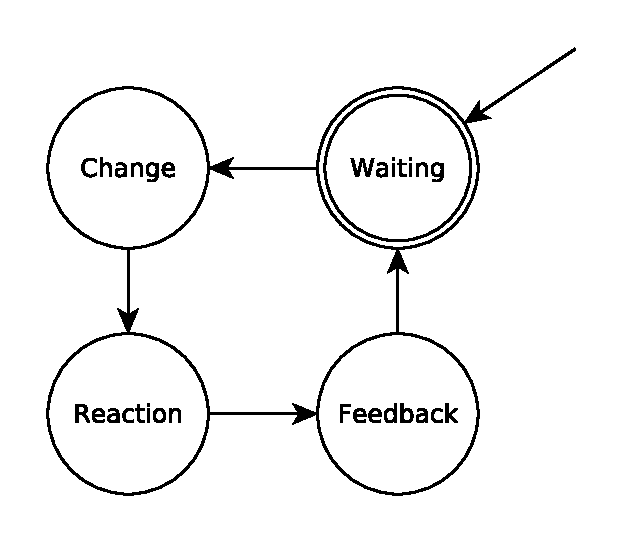
\includegraphics[scale=0.5]{eps/stages_of_ci.eps}
		\end{figure}
	\end{multicols}
\end{frame}

\begin{frame}\frametitle{Automated Code Review}
	TODO
\end{frame}

\bluepage{Thank You For Your Attention !}

\end{document}
